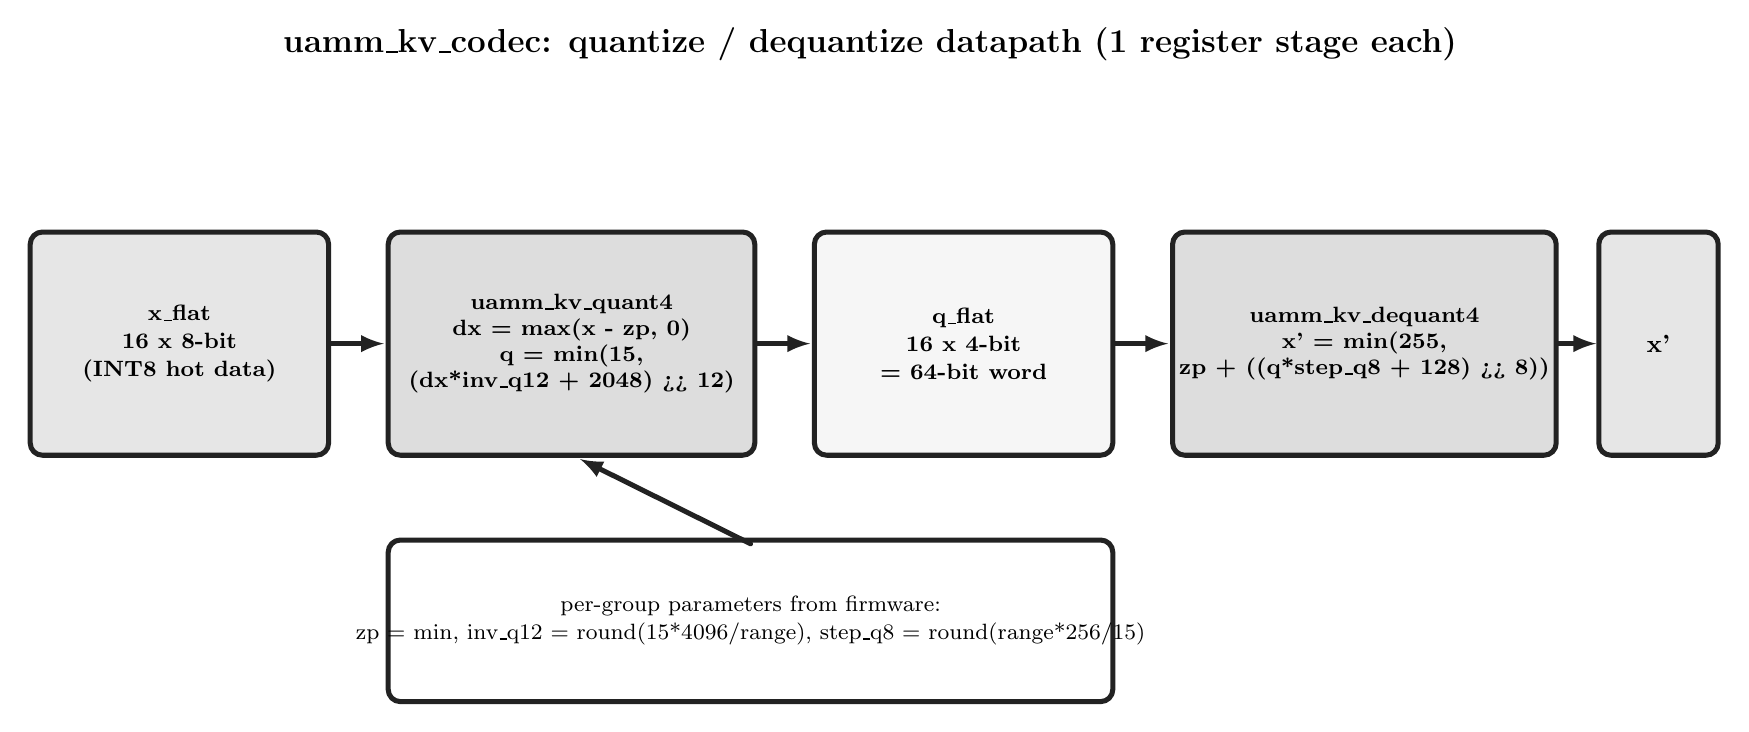
\begin{tikzpicture}[line cap=round,line join=round]
\draw[rounded corners=4.4pt,line width=1.82pt,draw={rgb,255:red,34;green,34;blue,34},fill={rgb,255:red,230;green,230;blue,230}] (0.064in,1.521in) rectangle (1.556in,2.637in);
\draw[rounded corners=4.4pt,line width=1.82pt,draw={rgb,255:red,34;green,34;blue,34},fill={rgb,255:red,221;green,221;blue,221}] (1.854in,1.521in) rectangle (3.687in,2.637in);
\draw[rounded corners=4.4pt,line width=1.82pt,draw={rgb,255:red,34;green,34;blue,34},fill={rgb,255:red,246;green,246;blue,246}] (3.985in,1.521in) rectangle (5.477in,2.637in);
\draw[rounded corners=4.4pt,line width=1.82pt,draw={rgb,255:red,34;green,34;blue,34},fill={rgb,255:red,221;green,221;blue,221}] (5.776in,1.521in) rectangle (7.694in,2.637in);
\draw[rounded corners=4.4pt,line width=1.82pt,draw={rgb,255:red,34;green,34;blue,34},fill={rgb,255:red,230;green,230;blue,230}] (7.907in,1.521in) rectangle (8.504in,2.637in);
\draw[-latex,line width=1.82pt,draw={rgb,255:red,34;green,34;blue,34}] (1.560in,2.079in) -- (1.833in,2.079in);
\draw[-latex,line width=1.82pt,draw={rgb,255:red,34;green,34;blue,34}] (3.691in,2.079in) -- (3.964in,2.079in);
\draw[-latex,line width=1.82pt,draw={rgb,255:red,34;green,34;blue,34}] (5.482in,2.079in) -- (5.754in,2.079in);
\draw[-latex,line width=1.82pt,draw={rgb,255:red,34;green,34;blue,34}] (7.698in,2.079in) -- (7.894in,2.079in);
\draw[rounded corners=4.4pt,line width=1.82pt,draw={rgb,255:red,34;green,34;blue,34},fill={rgb,255:red,255;green,255;blue,255}] (1.854in,0.289in) rectangle (5.477in,1.097in);
\draw[-latex,line width=1.82pt,draw={rgb,255:red,34;green,34;blue,34}] (3.666in,1.078in) -- (2.813in,1.502in);
\node[align=center,text={rgb,255:red,0;green,0;blue,0},font=\fontsize{8.5pt}{10.0pt}\selectfont\bfseries,inner sep=0pt] at (0.810in,2.079in) {x\_flat \\ 16 x 8-bit \\ (INT8 hot data)};
\node[align=center,text={rgb,255:red,0;green,0;blue,0},font=\fontsize{8.0pt}{9.4pt}\selectfont\bfseries,inner sep=0pt] at (2.771in,2.079in) {uamm\_kv\_quant4 \\ dx = max(x - zp, 0) \\ q = min(15, \\ (dx*inv\_q12 + 2048) >> 12)};
\node[align=center,text={rgb,255:red,0;green,0;blue,0},font=\fontsize{8.5pt}{10.0pt}\selectfont\bfseries,inner sep=0pt] at (4.731in,2.079in) {q\_flat \\ 16 x 4-bit \\ = 64-bit word};
\node[align=center,text={rgb,255:red,0;green,0;blue,0},font=\fontsize{8.0pt}{9.4pt}\selectfont\bfseries,inner sep=0pt] at (6.735in,2.079in) {uamm\_kv\_dequant4 \\ x' = min(255, \\ zp + ((q*step\_q8 + 128) >> 8))};
\node[align=center,text={rgb,255:red,0;green,0;blue,0},font=\fontsize{9.0pt}{10.6pt}\selectfont\bfseries,inner sep=0pt] at (8.205in,2.079in) {x'};
\node[align=center,text={rgb,255:red,0;green,0;blue,0},font=\fontsize{8.5pt}{10.0pt}\selectfont,inner sep=0pt] at (3.666in,0.693in) {per-group parameters from firmware: \\ zp = min,  inv\_q12 = round(15*4096/range),  step\_q8 = round(range*256/15)};
\node[anchor=south,align=center,text={rgb,255:red,0;green,0;blue,0},font=\fontsize{12.0pt}{14.2pt}\selectfont\bfseries,inner sep=0pt] at (4.263in,3.490in) {uamm\_kv\_codec: quantize / dequantize datapath (1 register stage each)};
\end{tikzpicture}
